\chapter{Caso de aplicación}
\label{apendicecaso}
\section{Tratamiento de fracturas}

El tratamiento de fracturas inicia con el examen y diagnóstico de la lesión de un paciente. A consideración del especialista se puede o no requerir de un examen de rayos X. En este último caso, puede ser necesario uno o más procedimientos de: cirugía, fijación o yeso. 

Nótese que los diferentes procedimientos a seguir pueden ser únicos caminos según las líneas de dependencia o se pueden combinar entre sí según el juicio de los especialistas médicos. Por ejemplo, pudiera ocurrir que luego de la cirugía, se requiera una fijación o incluso antes de la cirugía se prescriba cabestrillo. Así que, solo existen las restricciones de inicio de tareas como por ejemplo, realizar cirugía, fijación y yeso dependen de rayos X; rayos X y prescribir cabestrillo dependen de examinar paciente; y prescribir rehabilitación depende de realizar cirugía.
\begin{figure}[htp]
	\centering
		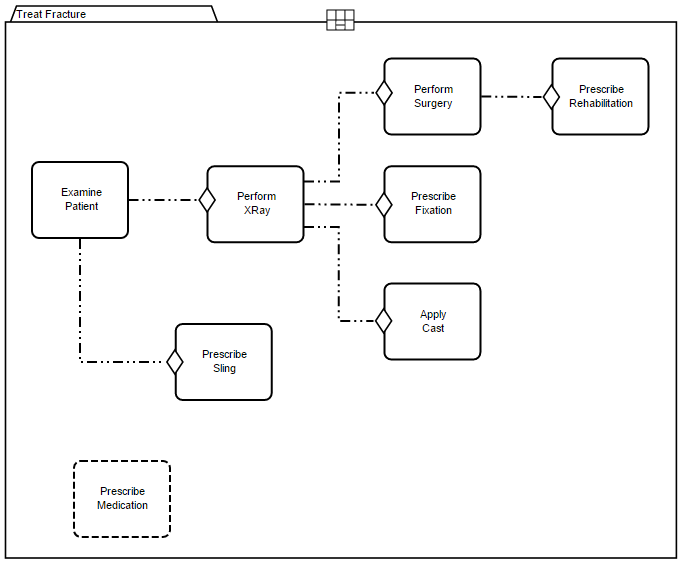
\includegraphics[width=12cm]{Fracturas1.png}
	\caption[Plan de caso para el tratamiento de fracturas]{Plan de caso para el tratamiento de fracturas. Fuente OMG CMMN}
	\label{fracturas1}
\end{figure}

De este caso, en la figura \ref{fracturas1} tenemos que:
%\renewcommand{\labelenumi}{\ref{apendicecaso}.}
%\renewcommand{\labelenumii}{\theenumii}
%\renewcommand{\theenumii}{\theenumi.\arabic{enumii}.}

\begin{enumerate}
    
\item Claramente, el proceso inicia con el examen de la situación del paciente o diagnóstico 

\item Una vez finalizado el examen se puede prescribir un cabestrillo, u ordenar una placa de RX para determinar la magnitud de la fractura

\item De acuerdo con la severidad de lesión, determinada una vez leídas las placas uno o más de tres procedimientos, se pueden iniciar, como son:

\begin{itemize}
    \item Prescribir fijación (quietud), para que suelden los huesos 
    \item Aplicar yeso
    \item Practicar cirugía, en el caso más grave
\end{itemize}

\item Por lo general, cuando se realiza cirugía, es necesario prescribir rehabilitación

\item Finalmente, en cualquier caso, puede ser necesario prescribir medicamentos.
\end{enumerate}

El modelo como tal, no define secuencia alguna entre las diferentes tareas, solo se condiciona el inicio de algunas tareas a la terminación de alguna otra tarea. Por lo tanto, la secuencia (flujo) solo se puede determinar una vez finalizada una instancia. 



